\section{Corredores de aproximação e zonas de segurança}
\label{sec:corredores_kozs}

A aproximação ocorre ao longo do eixo radial do alvo (R-bar), e utiliza um cone de aproximação alinhado com esse eixo e uma \textit{keep-out zone} (KOZ) no formato de uma elipsoide em torno da porta de acoplamento.

\begin{figure}[ht]
    \label{fig:corredor_app}
\centering
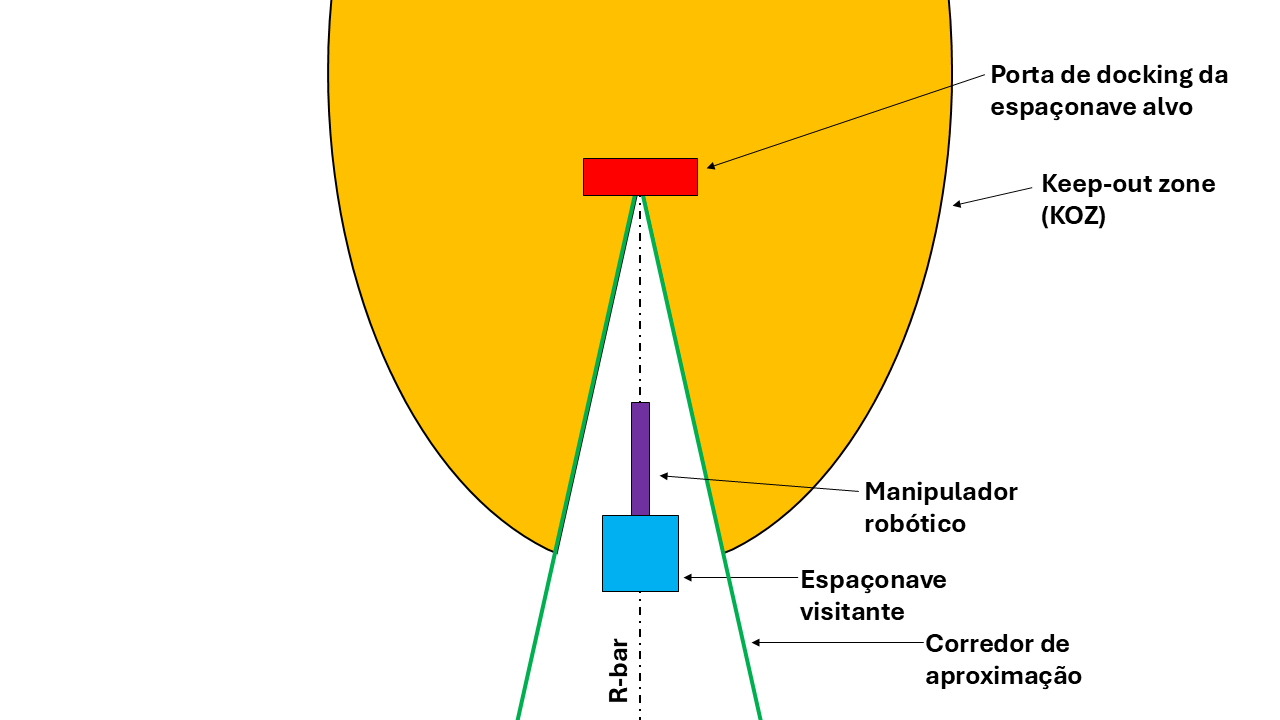
\includegraphics[width=1\linewidth]{3 Estrategia de RVDB/Imagens/2 Corredor e KOZ.png}
\caption{Corredor de aproximação e Keep-out zone.}
\end{figure}

\subsection{Corredor de aproximação}

Considerando o referencial LVLH do alvo, sendo seu eixo $x$ alinhado longitudinalmente no eixo radial (R-bar), $y$ alinhado com o vetor velocidade (\emph{along-track}) orbital e $z$ no eixo normal ao plano orbital.
O visitante deve permanecer em todo o tempo dentro do corredor de aproximação.

\subsection{Zona de exclusão}

A \emph{Keep-out Zone} (KOZ) de formato elipsoidal em torno da porta de acoplamento é utilizada como uma região proíbida onde o visitante não pode estar pois interfere na segurança da missão. Nessa região existe o risco do visitante colidir com outras partes físicas da espaçonave alvo.

\subsection{Infração da KOZ}

Caso o visitante entre na zona de exclusão, a aproximação final (ou curta) será abortada e o veículo deverá retornar ao ponto de espera anterior e realizar novas checagens.


